% UTF-8 encoding
% Compile with latex+dvipdfmx, pdflatex, xelatex or lualatex

\documentclass[hyperref, UTF8]{ctexart}
\usepackage{graphicx}
\usepackage{amssymb}
\usepackage{amsmath}
\usepackage{subfigure}
\usepackage{geometry}
\usepackage{caption}
\usepackage{upgreek}
\newcommand{\volt}{{\rm V}}
\newcommand{\source}{{\rm S}}
\newcommand{\ampere}{{\rm A}}
\newcommand{\milliampere}{{\rm mA}}
\newcommand{\hertz}{{\rm Hz}}
\newcommand{\kilohertz}{{\rm kHz}}
\newcommand{\megahertz}{{\rm MHz}}
\newcommand{\ohm}{\Omega}
\newcommand{\kiloohm}{{\rm k}\Omega}
\newcommand{\watt}{{\rm W}}
\newcommand{\kilowatt}{{\rm kW}}
\newcommand{\degree}{^{\circ}}
\newcommand{\farad}{{\rm F}}
\newcommand{\microfarad}{{\rm \upmu F}}
\newcommand{\millifarad}{{\rm mF}}
\newcommand{\henry}{{\rm H}}
\newcommand{\decibel}{{\rm dB}}
\newcommand{\J}{{\rm j}}

\title{电子学基础——第二次仿真作业}
\author{LXQ}
\date{2019.11.22}

\geometry{left=2.0cm, right=2.0cm, top=2.5cm, bottom=2.5cm}
\linespread{1}

\begin{document}

\maketitle

\paragraph{1} Using ac analysis in Multisim, plot the frequency response of the circuit depicted in Fig. 8-68.

\paragraph{答}
仿真电路图以及仿真所得到的幅频和相频特性曲线如图所示。由图可知,在低频($1\megahertz$以下)时,电路的作用为移相器,且所移动相位为$\pi$。当频率逐渐增高,电路的移相作用趋于$0$。

\begin{figure}[!htb]
    \centering
    \begin{minipage}[t]{0.346\textwidth}
    \centering
    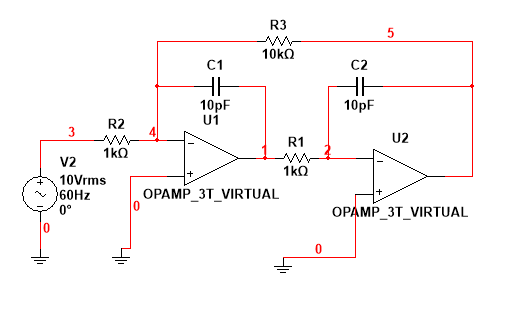
\includegraphics[width=1\textwidth]{cir.png}
    \caption*{(1) 电路图}
    \end{minipage}
    \\
    \begin{minipage}[t]{0.453\textwidth}
    \centering
    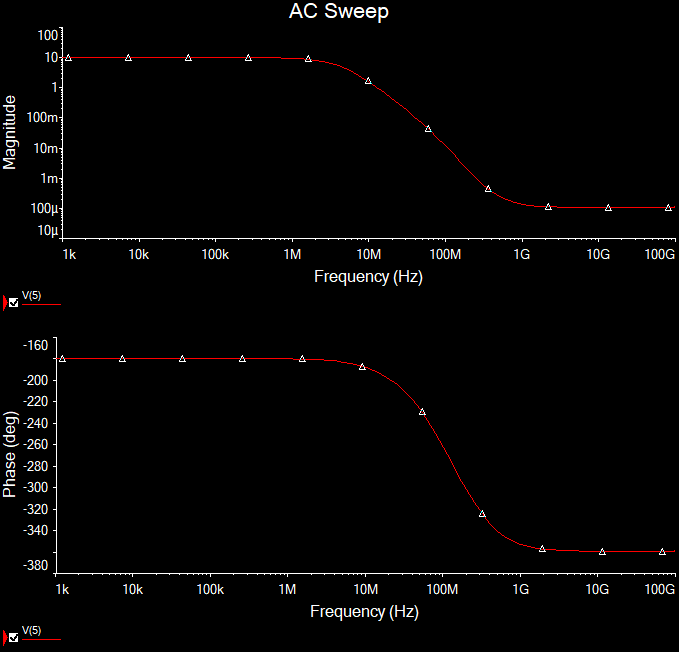
\includegraphics[width=1\textwidth]{res.png}
    \caption*{(2) 仿真结果}
    \end{minipage}
    \caption*{Figure 1}
\end{figure}    

\end{document} 